\documentclass{report}
\usepackage{pdfpages}
\usepackage{graphicx} 
\usepackage{dirtytalk}
\usepackage{lmodern}
\usepackage{booktabs}
\usepackage{listings}
\usepackage{float}
\usepackage{siunitx}
\usepackage{amsmath}
\usepackage{rotating}
\usepackage{arydshln}
\usepackage[hidelinks]{hyperref}
\usepackage[ngerman]{babel}
\usepackage[a4paper, total={6in, 8in}]{geometry}
\begin{document}

\includepdf[pages=-]{./PDFs/Deckblatt_P1}
\begin{titlepage}
    \begin{center}
        \vspace*{1cm}
            
        \Huge
        \textbf{Auswertung und Protokoll}
            
        \vspace{0.5cm}
        \LARGE
        Zum Versuch ROT - Rotationsbewegungen
        
        \vspace{1.8cm}

        \textbf{Jonas Müther \& Alejandro Schultheiss}
        \vfill
            
        P1 Praktikum\\
       
            
        \vspace{0.8cm}
  

        \vspace{1.8cm}
        \Large
        LMU München \\
        Physik B.Sc.\\
        Deutschland\\
        2026
            
    \end{center}
\end{titlepage}
\tableofcontents

\newpage
\chapter{Vorbereitung}

\section{Versuchsvorbereitung und Grundlagen des Versuchs}
\includepdf[pages=-]{./PDFs/VorbereitungROT.pdf}

\section{Versuchsprotokoll}
\includepdf[pages=-]{./PDFs/ROT_Versuchsdurchfuehrung.pdf}

\newpage
\chapter{Auswertung}
\section{Teilversuch I:}

\newpage
\section{Teilversuch II:}

\newpage
\section{Teilversuch III: Trägheitsmomente verschiedener Körper}
\subsection{Kalibrierung des Torsionspendels}
Aus den gemessenen Dauern für 5 Perioden ergeben sich die Periodendauern durch
\begin{equation}
    T = \frac{t_{ges}}{5}
\end{equation}
Daraus ergibt sich explizit mit den experimentell bestimmten Zeiten:
\begin{equation}
    \begin{split}
        T_1 &= \frac{78,7s}{5} = 15.740s \\
        T_2 &= \frac{78,9s}{5} = 15.780s \\
        \bar{T} &= \frac{T_1 + T_2}{2} = 15.760s
    \end{split}
\end{equation}
Die Unsichherheit errechnet sich folgendermaßen
\begin{equation}
    \begin{split}
        \Delta T = \frac{|T_1 - T_2|}{2} = 0.020s
    \end{split}
\end{equation}
Somit folgt:
\begin{equation}
    \begin{split}
        T = 15.760 \pm 0.020s
    \end{split}
\end{equation}
Für die Kalibrierungsscheibe wurden außerdem folgende Messwerte bestimmt:
\begin{equation}
    \begin{split}
        m_s &= 3.0117 \pm 0.0002 \si{kg} \\
        R_s &= 84.75 \pm 0.25 \si{mm} 
    \end{split}
\end{equation}
Aus diesen Werten kann nun der Kalibrierfaktor $K = \frac{D_{\phi}}{4\pi^2}$ hierzu wird Formel 10 aus dem Skript verwendet.
\begin{equation}
    \begin{split}
        T^2 &= 4 \pi^2 \frac{I}{D_{\phi}} \\
        \Leftrightarrow \bar{\frac{D_{\phi}}{4 \pi^2}} &= \frac{I}{T^2} \\
        \Leftrightarrow \bar{K} &= \frac{\frac{1}{2}m_s R_s^2}{T^2} \\
        \Leftrightarrow \bar{K} &= \boxed{\qty{4.355e-5}{Nm}}
    \end{split}
\end{equation}
Die Unsicherheit des Kalibrierfaktors  errechnet sich durch Gaußsche Fehlerfortpflanzung:
\begin{equation}
    \begin{split}
        \Delta K &= \sqrt{\left(\frac{\partial K}{\partial T} \Delta T\right)^2 + \left(\frac{\partial K}{\partial m} \Delta m\right)^2 + \left(\frac{\partial K}{\partial R} \Delta R\right)^2}\\
                 &= \sqrt{\left(\frac{m_s R_s^2}{T^3} \Delta T\right)^2 + \left(\frac{\frac{1}{2} R_s^2}{T^2} \Delta m\right)^2 + \left(\frac{m_s R_s}{T^2} \Delta R_s\right)^2} \\
        \Rightarrow \frac{\Delta K}{K} &= \sqrt{\left(2\frac{\Delta T}{T}\right)^2 + \left(\frac{\Delta m}{m}\right)^2 + \left(2\frac{\Delta R}{R}\right)^2} \\
                                       &= \qty{6.457e-3}{} \\
        \Rightarrow \Delta K &= \frac{\Delta K}{K} \cdot \bar{K} \approx \boxed{\qty{2.9e-7}{Nm}}
    \end{split}
\end{equation}
Somit ergibt sich für den Kalibrierfaktor:
\begin{equation}
    \begin{split}
        \boxed{\frac{D_{\phi}}{4\pi^2} = (4.355 \pm 0.029) \times 10^{-5} \si{Nm}}
    \end{split}
    \label{eq:Kalibrierfaktor}
\end{equation}
\subsection{Experimentelle Trägheitsmomente für verschiedene Quaderachsen}
Im Versuch wurden die Dauern für jeweils 5 Schwingungen am Torsionspendel für verschiedene Achsen eines Quaders jeweils 2 mal pro Achse bestimmt. 
Die Achsen sind nach der Grafik \ref{fig:AchsenQuader} nummeriert.
\begin{figure}[H]
    \centering
    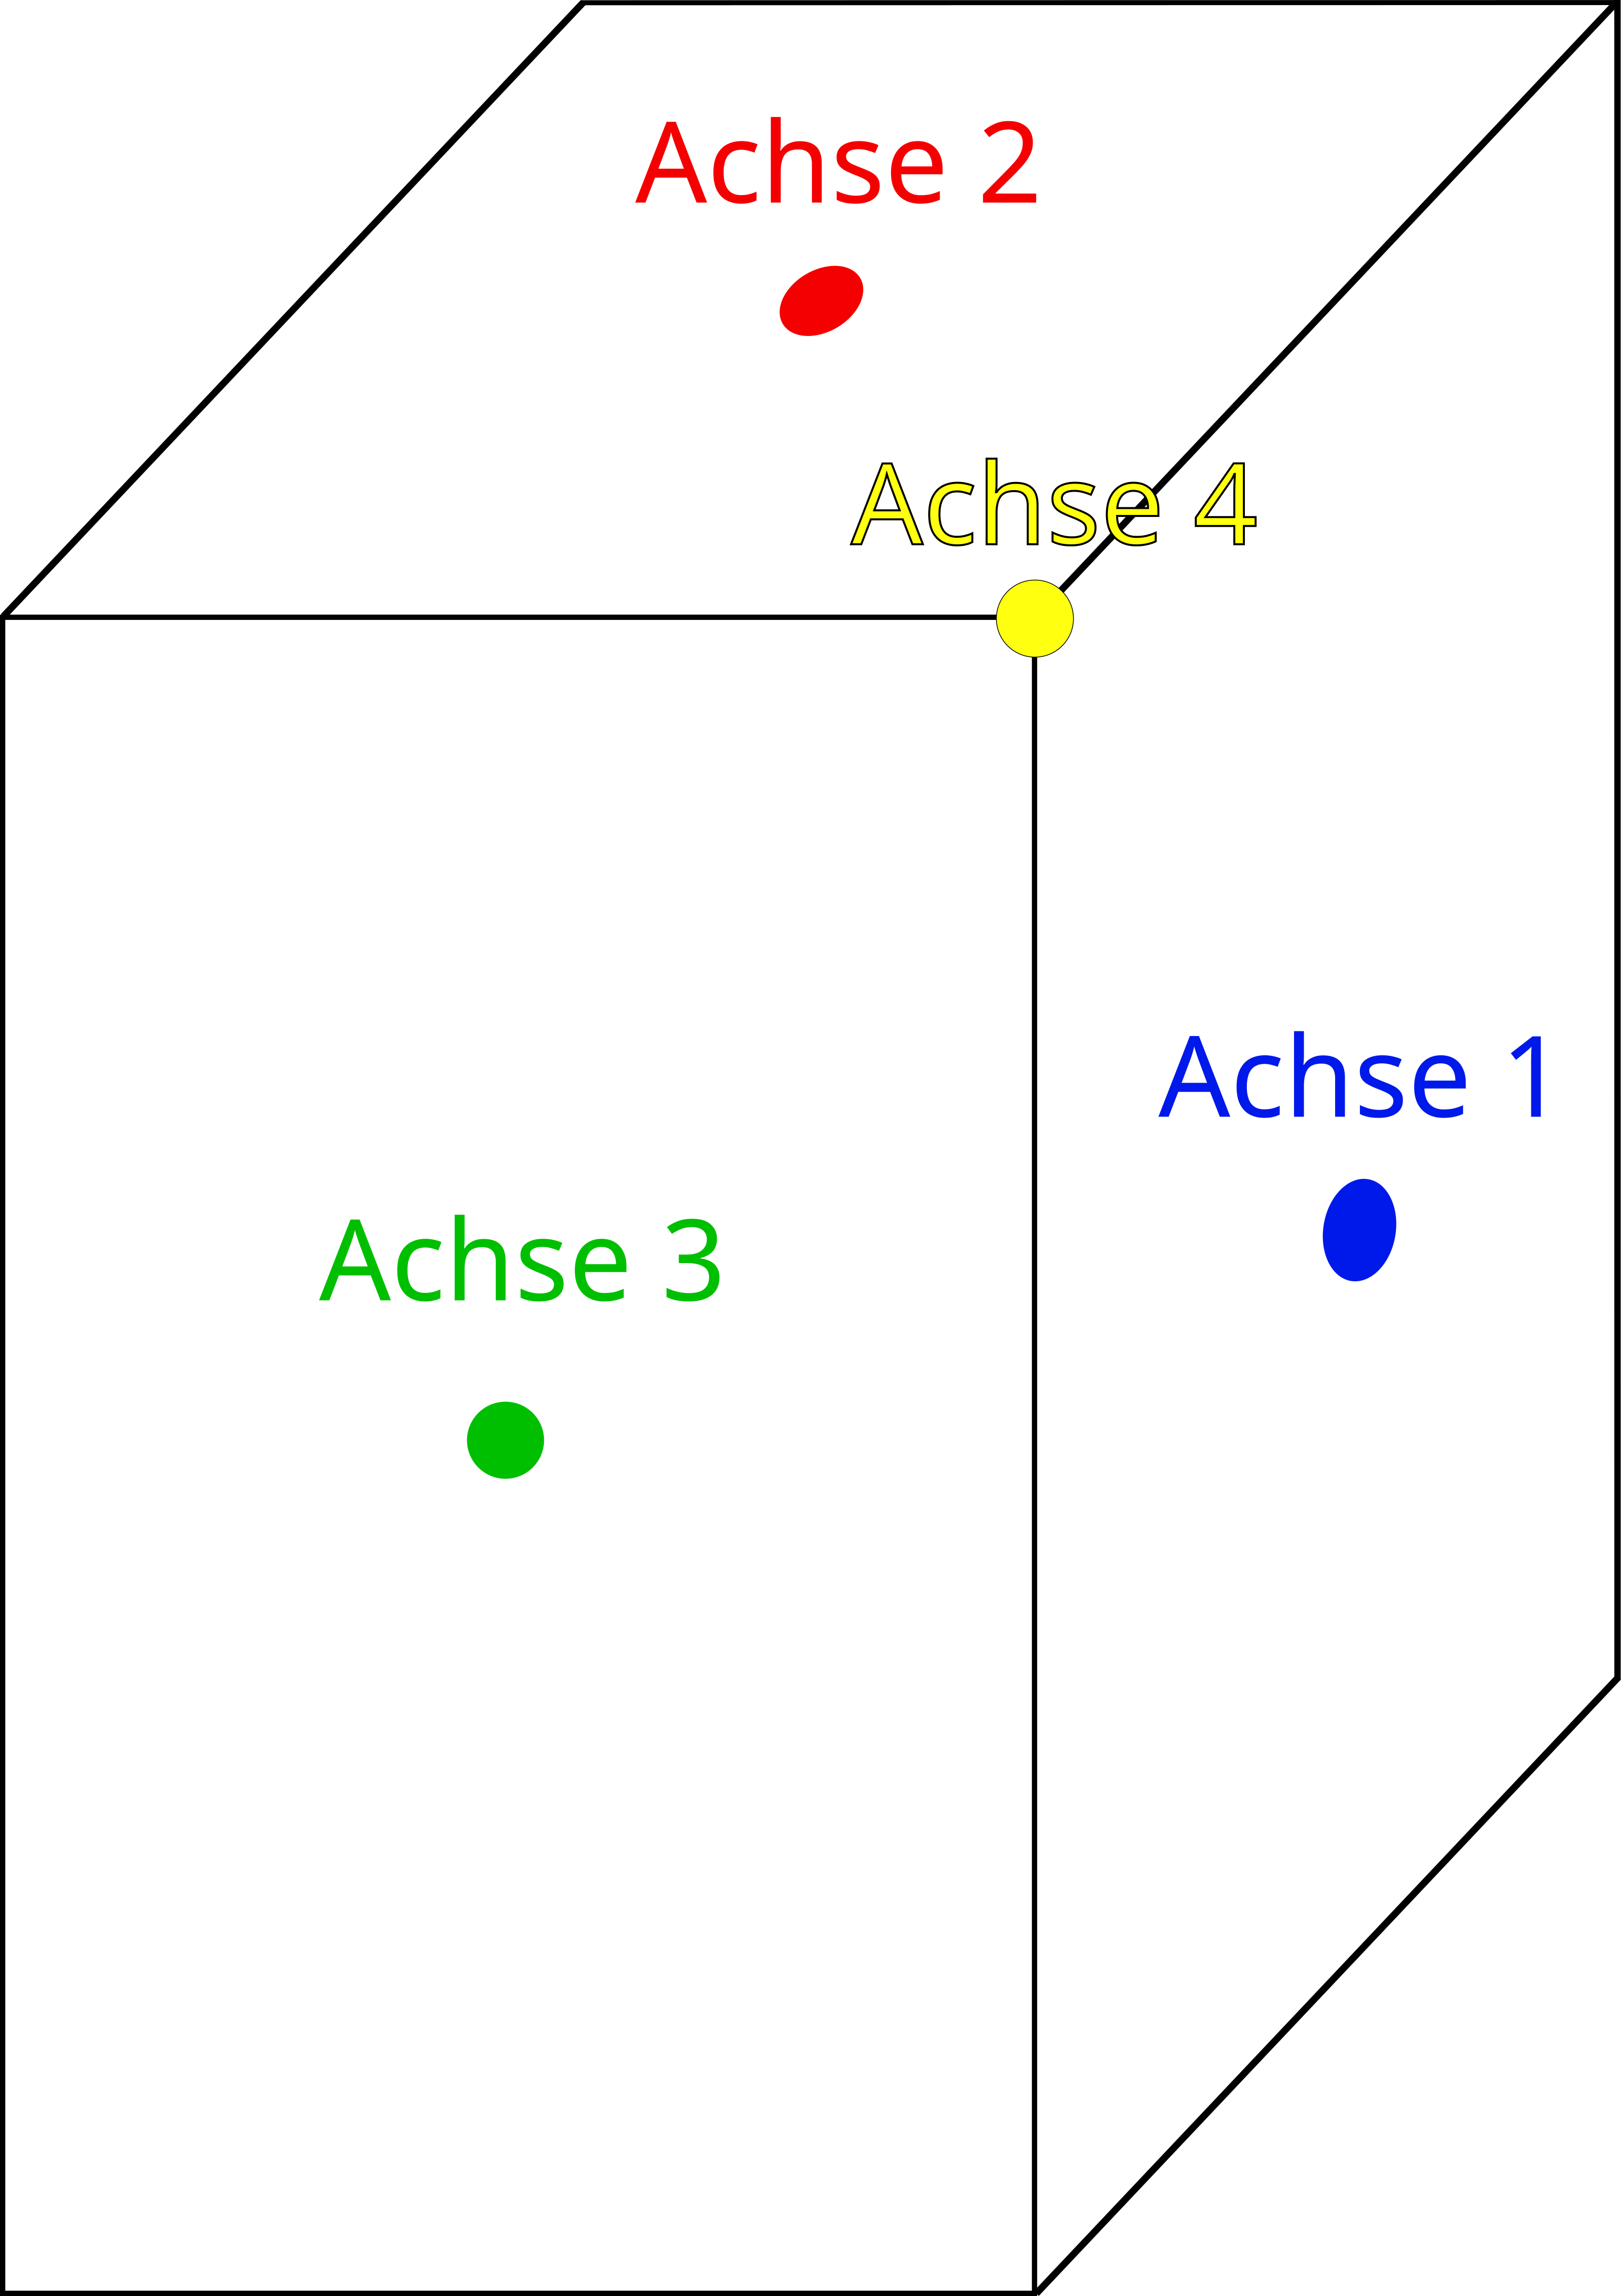
\includegraphics[width=.4\textwidth]{./Images/AchsenQuader.png}
    \caption{Achsen des Quaders}
    \label{fig:AchsenQuader}
\end{figure}
Aus den Dauern für 5 Schhwingungen können die Periodendauern jede Achse $i$ inkl Fehler analog zur Berechnung für das Kalibrierungspendel bestimmt werden. Hierzu werden die Formeln \ref{eq:Periodendauern} verwendet.
\begin{equation}
    \begin{split}
        \bar{T}_i &= \frac{t_{i1} + t_{i2}}{10} \\
        \Delta T_i &= \frac{|T_{i1} - T_{i2}|}{2} \\
        T_i &= \bar{T}_i \pm \Delta T_i
    \end{split}
    \label{eq:Periodendauern}
\end{equation}
Durch Einsetzen der gemessenen Werte ergeben sich die folgenden Periodendauern für die einzelnen Achsen:
\begin{equation}
    \begin{split}
        T_1 &= (9.66 \pm 0.13)\si{s} \\
        T_2 &= (6.82 \pm 0.16)\si{s} \\
        T_3 &= (8.79 \pm 0.15)\si{s} \\
        T_4 &= (7.90 \pm 0.04)\si{s} 
    \end{split}
\end{equation}
Daraus können mithilfe der Formel (10) aus dem Skript die Trägheitsmomente berechnet werden. Diese wird in Formel \ref{eq:Traegeitsmoment} nach I umgestellt.
\begin{equation}
    \begin{split}
        T^2 &= 4 \pi^2 \frac{I}{D_{\phi}} \\
        \Leftrightarrow I &= T^2 \frac{D_{\phi}}{4 \pi^2}
    \end{split}
    \label{eq:Traegeitsmoment}
\end{equation}
Setzt man die Werte Periodendauern, sowie den zuvor bestimmten Kalibrierfaktor \ref{eq:Kalibrierfaktor} ein, erhält man folgende Trägheitsmomente für die 
vier Achsen:
\begin{equation}
    \begin{split}
        \bar{I}_1 &= \qty{4.0635e-3}{kg \cdot m^2} \\
        \bar{I}_2 &= \qty{2.0254e-3}{kg \cdot m^2} \\
        \bar{I}_3 &= \qty{3.3645e-3}{kg \cdot m^2} \\
        \bar{I}_4 &= \qty{2.7177e-3}{kg \cdot m^2} \\
    \end{split}
\end{equation}
Die Unsicherheit ist gegeben durch:
\begin{equation}
    \begin{split}
        \frac{\Delta I}{I} &= \frac{1}{I} \sqrt{\left(\frac{\partial I}{\partial T} \Delta T\right)^2 + \left(\frac{\partial I}{\partial K}\Delta K\right)^2} \\
                           &= \sqrt{\left(2\frac{\Delta T}{T}\right)^2 + \left(\frac{\Delta K}{K}\right)^2}
    \end{split}
\end{equation}
mit $\Delta I = \frac{\Delta I}{I} \cdot \bar{I}$ ergibt sich für die einzelnen Unsicherheiten:
\begin{equation}
    \begin{split}
        \Delta I_1 &= \qty{0.12e-3}{kg \cdot m^2} \\
        \Delta I_2 &= \qty{0.09e-3}{kg \cdot m^2} \\
        \Delta I_3 &= \qty{0.12e-3}{kg \cdot m^2} \\
        \Delta I_4 &= \qty{0.04e-3}{kg \cdot m^2} \\
    \end{split}
\end{equation}
Zusammenfassend ergibt sich dann also für die Trägheitsmomente:
\begin{equation}
    \boxed{
        \begin{aligned}
        I_1 &= (4.06 \pm 0.12) \times 10^{-3} \si{kg \cdot m^2} \\
        I_2 &= (2.03 \pm 0.09) \times 10^{-3} \si{kg \cdot m^2} \\
        I_3 &= (3.36 \pm 0.12) \times 10^{-3} \si{kg \cdot m^2} \\
        I_4 &= (2.72 \pm 0.04) \times 10^{-3} \si{kg \cdot m^2}
        \end{aligned}
    }
    \label{eq:TraegeitsmomenteExp}
\end{equation}
\subsection{Trägheitsmoment der Diagonalen aus Hauptträgheitsmomenten}
Alternativ kann das Trägheitsmoment für Achse 4 aus den Trägheitsmomenten der Hauptachsen ($I_1, I_2, I_3$) berechnet werden.
Hierzu konstruiert man den Einheitsvektor $\vec{e}_d$, der in Richtung der Diagonalen des Quaders zeigt. (In Richtung der Achse 4)
Dieser lässt sich schreiben als $\vec{e} = a\vec{e}_1 + b\vec{e}_2 + c\vec{e}_3$. Die Vektoren $\vec{e}_i$ repräsentieren hier die Einheitsvektoren
in Richtung der Hauptachsen.
Mit den Komponenten $a, b, c$ kann das Trägheitsmoment entlang der Achse in Richtung $\vec{e}_d$ berechnet werden.
Dabei gilt die Formel:
\begin{equation}
    I_d = a^2I_1 + b^2I_2 + c^2I_3
    \label{eq:TraeghDiag}
\end{equation}
Laut Strahlensatz gilt:
\begin{equation}
    \frac{a}{||e_d||} = \frac{L_1}{L_d}, \qquad \frac{b}{||e_d||} = \frac{L_2}{L_d}, \qquad \frac{c}{||e_d||} = \frac{L_3}{L_d}
\end{equation}
Da per Definition $||e_d|| = 1$ und da $L_d^2 = L_1^2 + L_2^2 + L_3^2$, folgt:
\begin{equation}
    a^2 = \frac{L_1^2}{L_1^2 + L_2^2 + L_3^2}, \qquad b^2 = \frac{L_2^2}{L_1^2 + L_2^2 + L_3^2}, \qquad c^2 = \frac{L_3^2}{L_1^2 + L_2^2 + L_3^2}
    \label{eq:kompDiagvek}
\end{equation}
Somit gilt mit den Gleichungen \ref{eq:TraeghDiag} und \ref{eq:kompDiagvek}:
\begin{equation}
    I_d = \frac{L_1^2 I_1 + L_2^2 I_2 + L_3^2 I_3}{L_1^2 + L_2^2 + L_3^2}
    \label{eq:DiagFormel}
\end{equation}
Die Messwerte für die Längen $L_i$ sind:
\begin{equation}
    \begin{split}
        L_1 &= (51.50 \pm 0.03)mm \\
        L_2 &= (103.15 \pm 0.03)mm \\
        L_3 &= (72.95 \pm 0.03)mm \\
    \end{split}
\end{equation}
Einsetzen dieser Werte, sowie der Trägheitsmomente $I_i$ ergibt:
\begin{equation}
    \bar{I}_d = \qty{2.6995e-3}{kg \cdot m^2}
\end{equation}
Nun kann wiederrum die Gaußsche Fehlerfortpflanzung verwendet werdenn, um die Unsicherheit der Messwerte zu ermitteln.
\begin{equation}
\label{eq:UnsDiag}
\begin{split}
&\Delta I_d\\
&= \sqrt{
\left(\frac{\partial I_d}{\partial I_1}\Delta I_1\right)^2 +
\left(\frac{\partial I_d}{\partial I_2}\Delta I_2\right)^2 +
\left(\frac{\partial I_d}{\partial I_3}\Delta I_3\right)^2 +
\left(\frac{\partial I_d}{\partial L_1}\Delta L_1\right)^2 +
\left(\frac{\partial I_d}{\partial L_2}\Delta L_2\right)^2 +
\left(\frac{\partial I_d}{\partial L_3}\Delta L_3\right)^2
} \\[1ex]
&= \frac{1}{L_d^2} 
\sqrt{%
\begin{aligned}
& (L_1^2 \Delta I_1)^2 + (L_2^2 \Delta I_2)^2 + (L_3^2 \Delta I_3)^2 \\ 
&+ (2 L_1 (I_1 - I_d) \Delta L_1)^2 + (2 L_2 (I_2 - I_d) \Delta L_2)^2 + (2 L_3 (I_3 - I_d) \Delta L_3)^2
\end{aligned}%
} \\
&= \qty{0.064e-3}{kg \cdot m^2} \\
&\approx \qty{0.07e-3}{kg \cdot m^2} 
\end{split}
\end{equation}
Damit ergibt sich:
\begin{equation}
    \boxed{I_d = (2.70 \pm 0.07) \times 10^{-3} \si{kg \cdot m^2}}
    \label{eq:DiagTraegheitsmomentExpBer}
\end{equation}
Dieser berechnete Wert stimmt im Rahmen der Messungenauigkeit mit dem experimentell bestimmten Wert von $I_4 = 2.72\pm0.05$ überein.
($\bar{I}_d - \Delta I_d < \bar{I}_4 < \bar{I}_d + \Delta I_d$)

\subsection{Trägheitsmomente der Quaderachsen aus Geometrie}
Zuletzt ist es zudem möglich, die Trägheitsmomente ausschließlich aus den geometrischen Abmessungen und aus der Masse $m_Q = (3.0241 \pm 0.0002)kg$ zu bestimmten.
Mit dieser Methode erhält man folgende Ergebnisse:
\begin{equation}
    \begin{split}
        \bar{I}_{geom,1} &= \frac{1}{12}m(L_2^2 + L_3^2) \\
                         &= \qty{4.0225e-3}{kg \cdot m^2} \\
        \bar{I}_{geom,2} &= \frac{1}{12}m(L_1^2 + L_3^2) \\
                         &= \qty{2.0095e-3}{kg \cdot m^2} \\
        \bar{I}_{geom,3} &= \frac{1}{12}m(L_1^2 + L_2^2) \\
                         &= \qty{3.3497e-3}{kg \cdot m^2}                       
    \end{split}
\end{equation}
Die Unsicherheiten für diesen Fall ergeben sich durch Gauß'sche Fehlerfortpflanzung.
\begin{equation}
    \begin{split}
        \Delta I_{geom, i} &= \sqrt{\left(\frac{\partial I_{geom}}{\partial m} \Delta m\right)^2 + \left(\frac{\partial I_{geom}}{\partial L_j} \Delta L_j\right)^2 + \left(\frac{\partial I_{geom}}{\partial L_k} \Delta L_k\right)^2} \\
                           &= \sqrt{\left(\frac{I_{geom, i}}{m} \Delta m\right)^2 + \left(\frac{mL_j}{6} \Delta L_j\right)^2 + \left(\frac{m L_k}{6} \Delta L_k\right)^2}
    \end{split}
\end{equation}
Setzt man die Werte in die Gleichung ein erhält man die Unsicherheiten:
\begin{equation}
    \begin{split}
        \Delta I_{geom, 1} &= \qty{0.0020e-3}{kg \cdot m^2} \\
        \Delta I_{geom, 2} &= \qty{0.0014e-3}{kg \cdot m^2} \\
        \Delta I_{geom, 3} &= \qty{0.0018e-3}{kg \cdot m^2}
    \end{split}
\end{equation}
$\bar{I}_{geom, 4}$ kann dann wieder mithilfe der Formel \ref{eq:DiagFormel} berechnet werden. Mit dieser ergibt sich:
\begin{equation}
    \bar{I}_{geom, 4} = \qty{2.6855e-3}{kg \cdot m^2}
\end{equation}
Die Unsicherheit errechnet sich hier ebenfalls analog mithilfe von Formel \ref{eq:UnsDiag}. Setzt man die Werte ein erhält man:
\begin{equation}
    \Delta I_{geom, 4} = \qty{0.0011}{kg \cdot m^2}
\end{equation}
Gesammelt ergibt sich somit für die aus der Geometrie bestimmten Trägheitsmomente:
\begin{equation}
    \boxed{
        \begin{aligned}
            I_{geom, 1} &= (4.0225 \pm 0.0020) \times 10^{-3} \si{kg \cdot m^2} \\
            I_{geom, 2} &= (2.0095 \pm 0.0014) \times 10^{-3} \si{kg \cdot m^2} \\
            I_{geom, 3} &= (3.3497 \pm 0.0018) \times 10^{-3} \si{kg \cdot m^2} \\
            I_{geom, 4} &= (2.6855 \pm 0.0011) \times 10^{-3} \si{kg \cdot m^2}
        \end{aligned}
    }
\end{equation}
Vergleicht man die experimentell bestimmten Werte \ref{eq:TraegeitsmomenteExp} mit diesen theoretischen Werten, erkennt man, dass die Werte im Rahmmen der Unsicherheiten
gut miteinander übereinstimmen. Auch der Wert, der aus den experimentell bestimmten Messwerten für die Diagonale berechnet wurde \ref{eq:DiagTraegheitsmomentExpBer}, ist mit dem Theoriewert konsistent.

\begin{equation}
    \boxed{
        \begin{aligned}
            I_{geom, 1} = (4.0225 \pm 0.0020) \times 10^{-3} \si{kg \cdot m^2} &\simeq I_{exp,1} = (4.06 \pm 0.12) \times 10^{-3} \si{kg \cdot m^2}\\[6pt]
            I_{geom, 2} = (2.0095 \pm 0.0014) \times 10^{-3} \si{kg \cdot m^2} &\simeq I_{exp,2} = (2.03 \pm 0.09) \times 10^{-3} \si{kg \cdot m^2}\\[6pt]
            I_{geom, 3} = (3.3497 \pm 0.0018) \times 10^{-3} \si{kg \cdot m^2} &\simeq I_{exp,3} = (3.36 \pm 0.12) \times 10^{-3} \si{kg \cdot m^2}\\[6pt]
            I_{geom, 4} = (2.6855 \pm 0.0011) \times 10^{-3} \si{kg \cdot m^2} &\simeq I_{exp,4} = (2.72 \pm 0.04) \times 10^{-3} \si{kg \cdot m^2}\\
                                                                               &\simeq I_d = (2.70 \pm 0.07) \times 10^{-3} \si{kg \cdot m^2}
        \end{aligned}
    }
\end{equation}



\newpage
\section{Teilversuch IV: }

\newpage
\chapter{Anhang}
\section{SCRIPTS}

\definecolor{codegreen}{rgb}{0,0.6,0}
\definecolor{codegray}{rgb}{0.5,0.5,0.5}
\definecolor{codepurple}{rgb}{0.58,0,0.82}
\definecolor{backcolour}{rgb}{0.95,0.95,0.92}

\lstdefinestyle{matlab}{
    backgroundcolor=\color{backcolour},   
    commentstyle=\color{codegreen},
    keywordstyle=\color{magenta},
    numberstyle=\tiny\color{codegray},
    stringstyle=\color{codepurple},
    basicstyle=\ttfamily\footnotesize,
    breakatwhitespace=false,         
    breaklines=true,                 
    captionpos=b,                    
    keepspaces=true,                 
    numbers=left,                    
    numbersep=5pt,                  
    showspaces=false,                
    showstringspaces=false,
    showtabs=false,                  
    tabsize=2
}

\end{document}
